\subsection{Арифметическая иерархия.}
\textbf{Утверждение.} Любую формулу можно экивалентным образом записать так, чтобы все кванторы были в начале, а потом шла бескванторная формула.
\begin{proof}
   Для начала избавимся от импликаций (выразим их с помощью $\lor, \land, \lnot$). Затем просто разберем случаи для каждой связки: \begin{itemize}
        \item $(\forall x \, A) \lor B \equiv \forall x (A \lor B)$, так как $x$ в $B$ не входит (то же самое для $\land$).
        \item  $(\exists x \, A) \lor B \equiv \exists x (A \lor B)$ (то же самое для $\land$).
        \item $\lnot (\exists x  \, A) \equiv \forall x \, \lnot A$ (аналогично для $\land$).
    \end{itemize}
\end{proof} 

Сейчас мы будем классифицировать $k$-местные предикаты ($P: \mathcal{N}^k \to \{ 0, 1 \}$). 

Старутем с классов $\Sigma_0, \Pi_0$. Оба этих класса представляют разрешимые предикаты и связаны свойством, что в $\Pi_0$ лежат отрицания всех предикатов из $\Sigma_0$. Далее, для $k > 0$ имеем: \begin{itemize}
    \item $p \in \Sigma_k$ означает, что \[\exists Q \in \Pi_{k - 1} : \forall \bar{x} \; P(\bar{x}) = 1 \Leftrightarrow \exists y \, Q(\bar{x}, y) = 1 \]
    Тут $\bar{x}$ -- это вектор из переменных, а $y$ -- ровно одна переменная.
    \item $P \in \Pi_k$ означает, что \[ \exists Q \in \Sigma_{k - 1} : \forall \bar{x} \; P(\bar{x}) \Leftrightarrow \forall y \, Q(\bar{x}, y) = 1  \]
\end{itemize}

Давайте поймем, что из себя предсталяет класс $\Sigma_1$. 

\textbf{Утверждение.} Класс $\Sigma_1$ -- перечислимые придикаты.

\begin{proof}
    Согласно определению это предикаты $P(x) \equiv \exists y \; R(x, y)$, где $R$ -- разрешимый. Очевидно, что предикаты такого вида перечислимы, так как легко представить полуразрешающий алгоритм: будем просто перебирать $y$ и запускать алгоритм $R(x, y)$; если он выдаст 1, то и мы выдадим 1, иначе продолжим перебирать. 
    
    Осталось доказать, что любой перечислимый предикат можно представить в таком виде. Давайте воспринимать $R(x, y)$ как то, что мы запускаем полуразрешающий алгоритм на входе $x$ на $y$ шагов и выдаем 1, если он остановился. Тогда $R$ будет разрешимым, а условие $\exists y R(x, y)$ как раз и будет задавать полуразрешимость.  
\end{proof}

Класс $\Pi_1$ представляет коперечислимые предикаты -- то есть предикаты, которые соответствуют дополнениям перечислимых множеств.

\vspace{3mm}

Определение классов $\Sigma_k$ и $\Pi_k$ рекурсивное, однако, мы можем развернуть его, и вот, что получится: \begin{gather*}
    P \in \Sigma_k \Longleftrightarrow \exists R - \text{раз. предикат} : \forall x \; P(x) = 1 \Leftrightarrow \exists y_1 \, \forall y_2 \, \exists y_3 \dots y_k \; R(x, y_1, y_2, \dots, y_k) = 1 \\ \\
    P \in \Pi_k \Longleftrightarrow \exists R - \text{раз. предикат} : \forall x \; P(x) = 1 \Leftrightarrow \forall y_1 \, \exists y_2 \, \forall y_3 \dots y_k \; R(x, y_1, y_2, \dots, y_k) = 1 
\end{gather*}
То есть кванторы чередуются, начиная либо с $\exists$ для $\Sigma_k$, либо с $\forall$ для $\Pi_k$. Последний квантор определяется в зависимости от четности $k$.

\begin{conj}
    Все классы $\Sigma_k, \Pi_k$ образуют арифметическую иерархию.
\end{conj}

Свойства арифметической иерархии: \begin{enumerate}
    \item \[p \in \Sigma_k \Leftrightarrow \lnot p \in \Pi_k\] Возьмем развернутое определение и проотрицаем его. Тогда все кванторы поменяются на противоположные, а внутренний предикат проотрицается, но все еще будет разрешимым.
    \item \[ \Sigma_k \cup \Pi_k \subseteq \Sigma_{k+1} \cap \Pi_{k+1} \] Для доказательства этого свойства, надо доказать четыре включения: \[ \Sigma_k \in \Sigma_{k+1} \quad \Sigma_k \in \Pi_{k + 1} \quad \Pi_k \in \Sigma_{k+1} \quad \Pi_k \in \Pi_{k+1} \] Докажем первое. Что означает, что $P \in \Sigma_k:$ \[ P(x) = 1 \Leftrightarrow \exists y_1 \; \forall y_2 \dots y_k \; R(x, y_1, \dots, y_k) \] Давайте припишем в конец фиктивный квантор и переменную $y_{k+1}$ (квантор будет противоположен тому, что перед $y_k$). Предикат $R$ от него не зависит, значит, ничего не нарушится.
    
    Для доказательства второго надо в начало приписать $\forall y_0$. Третье и четвертое аналогично.

    Таким образом, мы получили такую картинку: 

    \begin{center}
        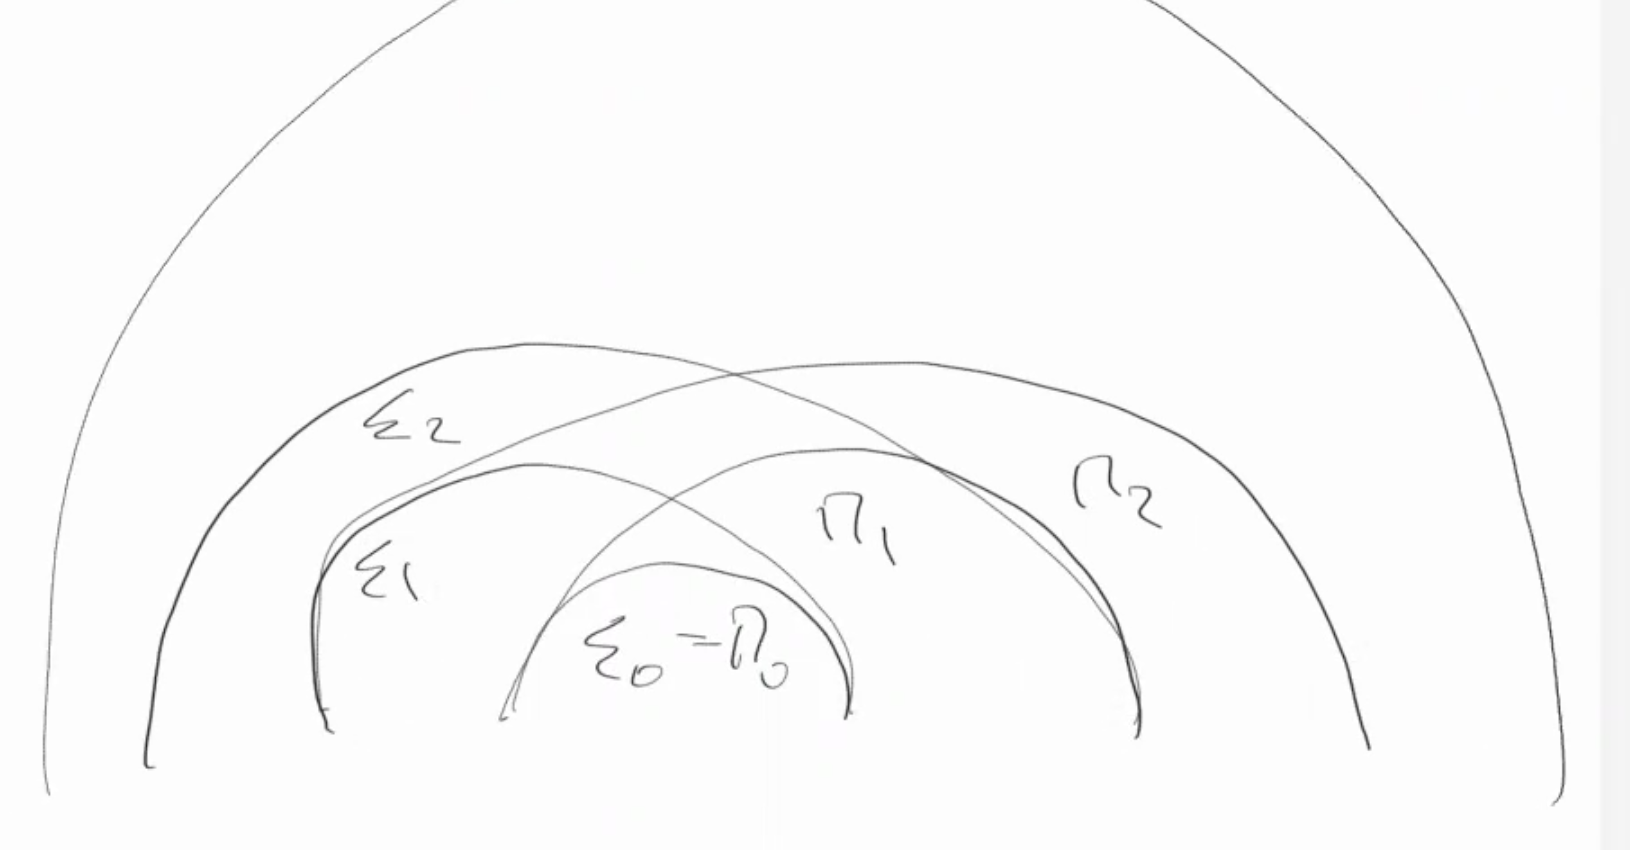
\includegraphics[scale=0.4]{ggwp.png}
    \end{center}
    

    \item Любой предикат, выразимый в арифметике, попадает в какой-то $\Sigma_k$ (и соответсвенно $\Pi_k$).
    
    Давайте вынесем все кванторы вперед (мы так умеем делать). После них останется бескванторная формула, которая является каким-то арифметическим выражением, следовательно, разрешима. Единственная проблема: кванторы могут не чередоваться. Она решается просто: добавим фиктивные переменные и кванторы, чтобы все начало чередоваться.
    \item Любой предикат из $\Sigma_k$ (и соответсвенно $\Pi_k$) выразим в арифметике. 
    
    Заметим, что предикат выглядит почти как формула: \[ P(x) = 1 \Leftrightarrow \exists y_1 \; \forall y_2 \dots y_k \; R(x, y_1, \dots, y_k) \] Надо только разобраться с $R(x, y_1, \dots, y_k)$. Это разрешимый предикат, следовательно перечислимый, а следовательно выразим в арифметике (теорема предыдущего параграфа). 

    \item $\Sigma_k$ и $\Pi_k$ замкнуты относительно $m$-сведений.
    
    Пусть $A \leqslant_m B$ и $B \in \Sigma_k$. Надо докзаать, что из этого следует, что $A \in \Sigma_k$. По определению: \[ B(x) = 1 \Leftrightarrow \exists y_1 \; \forall y_2 \dots y_k \; R(x, y_1, \dots, y_k) \]
    Тогда имеем \[ A(x) = 1 \Leftrightarrow B(f(x)) = 1 \Leftrightarrow \exists y_1 \; \forall y_2 \dots y_k \; R(f(x), y_1, \dots, y_k) \] Раз $f$ -- всюду определенная, вычислимая, разрешимость $R$ не нарушится. 
\end{enumerate}

\begin{conj}
    Пусть $S$ -- множество $k$-местных предикатов, $U(n, x_1, \dots, x_k)$ -- $(k+1)$-местный предикат. $U$ называется \textbf{универсальным} для $S$, если \[ \forall P \in S \; \exists n \in \mathcal{N} : P(x_1, \dots, x_k) = U(n, x_1, \dots, x_k) \]
\end{conj}

Продолжаем доказывать свойства: \begin{enumerate}
    \setcounter{enumi}{5}
    \item Введем предикат $U_{\Sigma_1}$: \[ U_{\Sigma_1}(n, \bar{x}) = 1 \Leftrightarrow \langle n \rangle (x) \text{ остановится} \]
    Заметим, что $U_{\Sigma_1} \in \Sigma_1$, так как он очевидно является перечислимым.

    Давайте докажем, что $(k+1)$-местный предикат $U_{\Sigma_1}$ -- универсальный предикат для множества $k$-местных предикатов $\Sigma_1$. Пусть $P$ -- $k$-местный предикат из $\Sigma_1$, тогда он является полуразрешимым. Зафиксируем $A$ -- полуразрешающий алгоритм для $P$. Тогда \[ P(x_1, \dots, x_k) = U(\#A, x_1, \dots, x_k) \]

    \item $U_{\Sigma_1}$ универсальный для $\Sigma_1 \Longrightarrow \lnot U_{\Sigma_1}$ универсальный для $\Pi_1$. Это следует из того, что в $\Pi_1$ лежат отрицания всех предикатов из $\Sigma_1$.
    \item $\forall k \geqslant 1$ и $\forall l \in \mathbb{N}$ в $\Sigma_k$ есть универсальный предикат для $l$-местных предикатов из $\Sigma_k$. Аналогично для $\Pi_k$ (это будет отрицания предиката для $\Sigma_k$).
    
    Будем доказывать сей занятный факт по индукции. Базу $k = 0$ мы уже доказали. Пусть теперь $P(x_1, \dots, x_l) \in \Sigma_{k+1}$. По определению \[ \exists Q \in \Pi_k : \forall x_1, \dots, x_l \;\; P(x_1, \dots, x_l) = 1 \Leftrightarrow \exists y \; Q(x_1, \dots, x_l, y) = 1 \] Возьмем универсальный предикат для $\Pi_k$ и подставим его в определение: \[ \exists q : \quad P(x_1, \dots, x_l) = 1 \Leftrightarrow \exists y \; U_{\Pi_k}(q, x_1, \dots, x_l, y) = 1 \] Тогда получаем, что \[ U_{\Sigma_{k+1}}(n, x_1, \dots, x_l) =   \exists y \; U_{\Pi_k}(n, x_1, \dots, x_l, y) \] Вместо $n$ мы будем подставлять $q$, что нашлось для предиката $U_{\Pi_k}$. 

    Казалось бы, что это лажа, но нет, мы дейтсвительно получили универсальный предикат. В зависимости от того, найдется ли $y$, при котором $U_{\Pi_k}(n, x_1, \dots, x_l, y)$ будет давать 1, мы будем получать значение нашего предиката.

    \item $\forall k \geqslant 0$ универсальный предикат для множества одноместных предикатов из $\Sigma_k$ не лежит в $\Pi_k$ (аналогично для $\Pi_k$ и $\Sigma_k$).
    
    Пусть $T(n, x)$ -- универсальный предикат для одноместных предикатов из $\Sigma_k$. От противного: пусть $T \in \Pi_k$. Возьмем $D(x) := T(x, x)$. Он тоже будет лежать в $\Pi_k$, так как переменные мы подставляем одинкаовые, поэтому количество кванторов не увеличится. Возьмем $S(x) = \lnot D(x)$, тогда $S(x) \in \Sigma_k$. Вспомним, что $T$ -- универсальный: \[ \exists s : S(x) = T(s, x) \forall x \]
    Подставим $s$ в $S$: \[ S(s) = T(s, s) = D(s) = \lnot S(s) \]
    Противоречие.

    \item Универсальный предикат для множества разрешимых предикатов не является разрешимым (следует из 9).
    \item $\Sigma_k \subsetneq \Sigma_{k+1}$ при $k \geqslant 1$ (на самом деле при $k = 0$ и так знаем, потому что перечислимые и разрешимые это не одно и то же).
    
    От противного. Пусть $\Sigma_k = \Sigma_{k+1}$. Знаем, что $\Sigma_{k+1} \supseteq \Pi_k$. Значит, $\Sigma_k$ содержит универсальный предикат для $\Pi_k$. Противоречие.
\end{enumerate}

Теперь мы готовы вывести предикат, не выразимый в арифметике (т.е. не лежащий ни в одном из $\Sigma_k$ или $\Pi_k$): \[ T = \{ n \,|\, \text{$n$ - номер замкнутой истинной формулы в арифметике} \} \] 
(Формально, мы задали множество, на котором предикат $T$ дает 1).

\vspace*{5mm}

\begin{theorem} (Тарского)
    Предикат $T$ не выразим в арифметике.
\end{theorem}
\begin{proof}
    От противного, пусть $T$ выразим, Тогда обязано выполняться, что $T \in \Sigma_k$ для какого-то $k$. Рассмотрим вспомогательное утверждение.

    \quad \textbf{Утверждение.} Если предикат $P$ выразим в арифметике, то $P$ сводится к $T$. 
    
    \quad \textbf{Доказательство.} Раз $P(x)$ выразим, то есть формула $\varphi(x)$, его считающая. Давайте 
    построим такое сведение: \[ \bar{X} \mapsto \#\varphi(\bar{x}), \] 
    где $\#\varphi(\bar{x})$ -- это номер формулы, в которой явно зашит $\bar{x}$ (вместо $x_i$ подставим $x_i$ единичек). Понятно, что это сведение, потому что $P$ истинно, когда $\varphi$ истинно, а с конкретной подстановкой это получается замкнутая формула, тогда ее номер лежит в $T$. 
    
    Вспоминаем, что мы доказывали, что $\Sigma_k$ и $\Pi_k$ замкнуты относительно сведений. Получаем, что любой выразимый в арифметике предикат $P \in \Sigma_k$. Давайте возьмем все такие $P$, по определнию лежащие в $\Sigma_{k+1}$. Получаем, что $\Sigma_{k+1} \subseteq \Sigma_k$. Противоречие.
\end{proof}

\begin{follow}
    $T$ не является перечислимым (очевидно, потому что мы доказывали, что все выразимые являются перечислимыми).
\end{follow}

Это так называемая \textbf{теорема Гёделя о неполноте}.

\vspace{5mm}

\begin{conj}
    Система доказательств для языка $L$ -- это алгоритм такой $\Pi$, что: \begin{itemize}
        \item $\Pi$ всегда останваливается,
        \item если $x \in L$, то существует такая строка $w$ (доказательство), что $\Pi(x, w) = 1$,
        \item если $\Pi(x, w) = 1$, то $x \in L$.
    \end{itemize}
\end{conj}

\begin{lemma}
    Для языка $L$ существует система доказательств $\Leftrightarrow$ язык $L$ перечислим.
\end{lemma}
\begin{proof} \quad \\
    $"\Rightarrow":$ перебираем все $w$ и запускаем $\Pi(x, w)$. Если хоть раз остановится, то выдадим $x$.

    $"\Leftarrow":$ знаем, что $x \in L \Leftrightarrow \exists y \; R(x, y)$, где $R$ -- разрешим. Тогда $y$ будет доказательством, а $R$ -- системой.
\end{proof}

\textbf{Альтернативное доказательсво, что предикат $T$ не перечислим.}

Вспомним про не перичислимое множество $\overline{W}$ -- множество таких $n$, что $\langle n \rangle (n)$ не останаваливается. Давайте сведем $\overline{W}$ к $T$: \[ n \mapsto \#"\forall t \; \langle n \rangle (n) \text{ не остан. за } t \text{ шагов}" \] Это работает, потому что предикат $"\langle n \rangle (n) \text{ не остан. за } t \text{ шагов}"$ разрешим, следовательно выражается в арифметике. Значит и выражение вида \[ \forall t \; \langle n \rangle (n) \text{ не остан. за } t \text{ шагов} \] записывается в арифметике. Остается только взять номер.